\documentclass{beamer}

\usepackage[utf8x]{inputenc}
\usepackage[OT4]{fontenc}

\usetheme[bullet=circle,
          titleline=true,
          pageofpages=of,
          alternativetitlepage=true]{Torino}

\usepackage{ragged2e}
\usepackage{hyphenat}
\usepackage{hyperref}
\usepackage{booktabs}

\usepackage{pgf,tikz}
\usepackage{pgfplots}

\usetikzlibrary{arrows}
\usetikzlibrary{automata}
\usetikzlibrary{backgrounds}
\usetikzlibrary{decorations}

\usepackage{amsmath}
\usepackage{amsfonts}
\usepackage{amsthm}

\definecolor{MyGreen}{rgb}{0.40,0.80,0.20}

\title{A New Online Interactive Web Notebook Based on ExtJS}
\author{Mateusz Paprocki \texttt{<mattpap@gmail.com>}}
\institute[PWR]{Wrocław University of Technology \newline University of Nevada, Reno}
\date{\today}

\newenvironment{jblock}[1]{
    \begin{block}{#1}\justifying\nohyphens
}{
    \end{block}
}

\setbeamercovered{transparent}

\begin{document}

\frame{\titlepage}

\begin{frame}
    \frametitle{Presentation plan}
    \framesubtitle{}

    \begin{itemize}
        %\item A few words about the speaker
        \item Classical user interfaces
        \pause
        \item Future plans
    \end{itemize}
\end{frame}

%\begin{frame}
%    \frametitle{A few words about the speaker}
%    \framesubtitle{}
%
%    \begin{center}
%        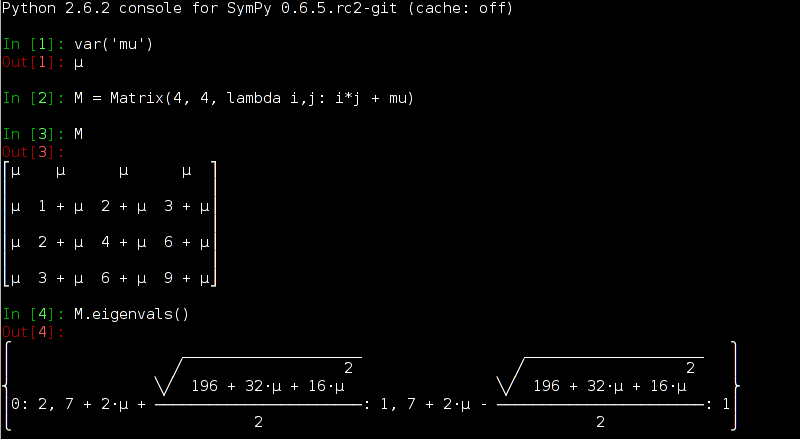
\includegraphics[scale=0.5]{images/sympy-unicode.png} % XXX
%    \end{center}
%
%    \begin{itemize}
%        \item on Friday graduated from Wrocław University of Technology
%    \end{itemize}
%\end{frame}

\begin{frame}
    \frametitle{Classical approaches to interactive UIs}
    \framesubtitle{A short introduction}

    \begin{itemize}
        \item \structure{terminal based} user interfaces
            \begin{itemize}
                \item single flow of inputs and outputs
                \item not easy to return to previous results
                \item primitive windowing possible via \texttt{curses} library
                \item often people consider black screen as something wrong
            \end{itemize}
        \item \structure{graphical} user interfaces
            \begin{itemize}
                \item take advantage of \structure{graphical toolkits}: Wx, GTK, Qt, \ldots
                \item much more \structure{user friendly} than terminal based UIs
            \end{itemize}
    \end{itemize}
\end{frame}

\begin{frame}
    \frametitle{Classical approaches to interactive UIs}
    \framesubtitle{Example: Terminal based user interfaces}

    \begin{center}
        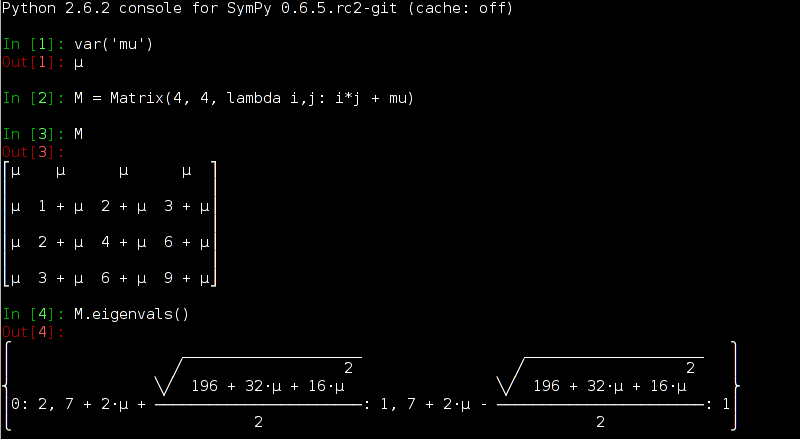
\includegraphics[scale=0.65]{images/sympy-unicode.png}
    \end{center}
\end{frame}

\begin{frame}
    \frametitle{Classical approaches to interactive UIs}
    \framesubtitle{Example: Graphical user interfaces}

    \begin{center}
        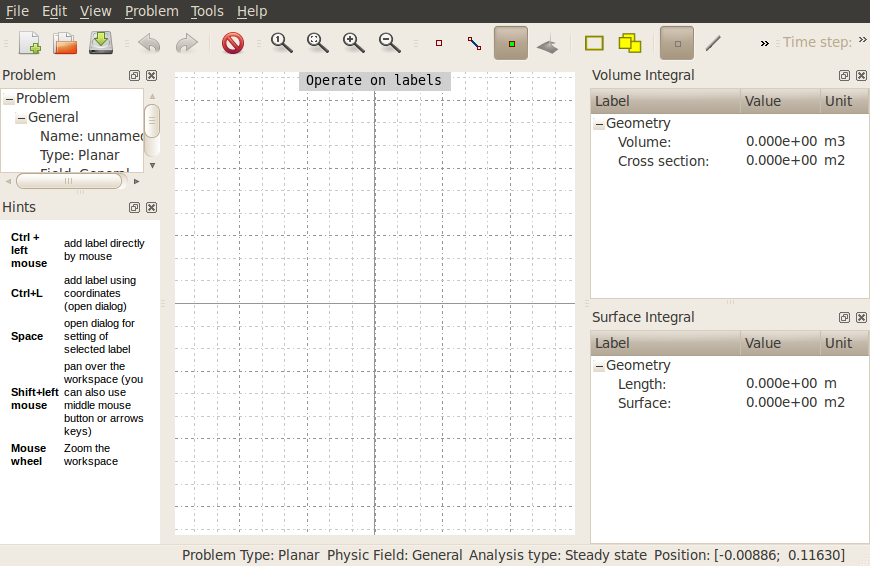
\includegraphics[scale=0.40]{images/agros2d-window.png}
    \end{center}
\end{frame}

\begin{frame}
    \frametitle{Classical approaches to interactive UIs}
    \framesubtitle{What is an alternative to this?}

    A \structure{web browser} based user interface:
    \begin{itemize}
        \item would run in a web browser: Firefox, Chrome, IE, \ldots
        \item no need to install any software on users' computers
            \begin{itemize}
                \item besides a web browser, but web browsers are \structure{pre--installed}
            \end{itemize}
    \end{itemize}
\end{frame}

\begin{frame}
    \frametitle{Classical approaches to interactive UIs}
    \framesubtitle{Advantages and disadvantages}

    {\color{MyGreen} Pros}:
    \begin{itemize}
        \item mainly benefits for developers
            \begin{itemize}
                \pause
                \item no problems with cross--browser compatibility
                \pause
                \item better tools: IDEs, debuggers, \ldots
                    \begin{itemize}
                        \pause
                        \item at least at the moment
                    \end{itemize}
            \end{itemize}
        \pause
        \item can take advantage of hardware
            \begin{itemize}
                \pause
                \item fast 2D and 3D visualisations
            \end{itemize}
    \end{itemize}
    \pause
    {\color{red} Cons}:
    \begin{itemize}
        \pause
        \item user needs to install the program
            \begin{itemize}
                \item different approaches for different platforms
                \item Internet access is needed to download the program
            \end{itemize}
        \pause
        \item in classroom we have to install on every machine
            \begin{itemize}
                \item a lot of effort required to setup all systems
                \item problems with keeping installations in sync
            \end{itemize}
    \end{itemize}
\end{frame}

\begin{frame}
    \frametitle{What is a web notebook?}
    \framesubtitle{}

    A solution to those problems is a \structure{web notebook}:
    \begin{itemize}
        \pause
        \item a program that can be run in most \structure{modern} web browsers
        \pause
        \item allows for executing source code (e.g. Python) on a web server
        \pause
        \item \structure{no need} for \structure{installation} on users' computers
        \pause
        \item takes advantage of \structure{centralized storage} on a web server
        \pause
        \item can be \structure{installed locally} if no network connection is available
    \end{itemize}
\end{frame}

\begin{frame}
    \frametitle{How a web notebook can be used?}
    \framesubtitle{}

    \begin{itemize}
        \item give interactive presentations, seminars, \ldots
            \begin{itemize}
                \pause
                \item prepare worksheets before your talk
                \pause
                \item show them together with slides
            \end{itemize}
        \pause
        \item teach your subject in a classroom
            \begin{itemize}
                \pause
                \item students can \structure{follow} your examples on their computers
                \pause
                \item you can include \structure{extended content} in your worksheets
                    \begin{itemize}
                        \pause
                        \item additional text, comments, theorems, \ldots
                        \pause
                        \item interactive components, applets, \ldots
                        \pause
                        \item videos and many other
                    \end{itemize}
                \pause
                \item students can run examples \structure{at home}, modify and extend them
                \pause
                \item you can prepare assignments and \structure{publish} them to your students
                \pause
                \item students can \structure{collaborate} on group projects
            \end{itemize}
    \end{itemize}
\end{frame}

\begin{frame}
    \frametitle{What is Codenode?}
    \framesubtitle{}

    An \structure{interactive} online \structure{notebook}:
    \begin{itemize}
        \pause
        \item implements multiple--level architecture
            \begin{itemize}
                \pause
                \item user web interface
                \pause
                \item frontend server
                \pause
                \item backend servers
            \end{itemize}
        \pause
        \item supports \structure{Python} and \structure{Sage}
        \pause
        \item uses a \structure{database} for storing worksheets and other data
        \pause
        \item available from \texttt{www.codenode.org}
    \end{itemize}
    \pause
    There are \structure{other} web interactive notebooks:
    \begin{itemize}
        \pause
        \item Sage Notebook (\texttt{www.sagenb.org}), \structure{\ldots}
    \end{itemize}
\end{frame}

\begin{frame}
    \frametitle{Codenode's Bookshelf}
    \framesubtitle{}

    \begin{center}
        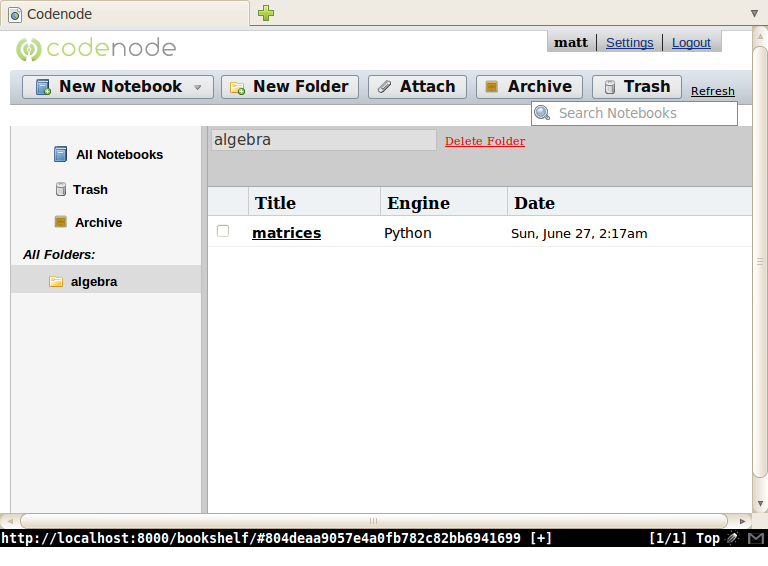
\includegraphics[scale=0.45]{images/codenode-bookshelf.png}
    \end{center}
\end{frame}

\begin{frame}
    \frametitle{Codenode's Worksheet}
    \framesubtitle{}

    \begin{center}
        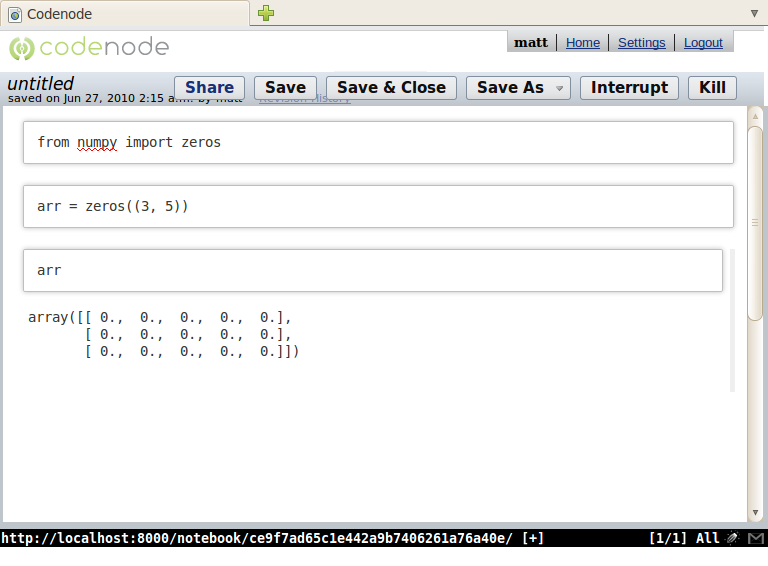
\includegraphics[scale=0.45]{images/codenode-worksheet.png}
    \end{center}
\end{frame}

\begin{frame}
    \frametitle{Codenode and Sage notebooks}
    \framesubtitle{The standard approach to web notebooks}

    \begin{itemize}
        \item \structure{single worksheet} per browser window (or tab)
            \begin{itemize}
                \pause
                \item not easy to show to different worksheets at once
            \end{itemize}
        \pause
        \item not easy to work with multiple worksheets in parallel
            \begin{itemize}
                \pause
                \item have to use multiple browser windows (or tabs)
            \end{itemize}
        \pause
        \item notebook UIs not embeddable in third--party web sites
            \begin{itemize}
                \pause
                \item no way to use a notebook embedded in your web site
            \end{itemize}
        \pause
        \item no well defined APIs for developers
            \begin{itemize}
                \pause
                \item not easy to replace a part of existing notebook
            \end{itemize}
    \end{itemize}
\end{frame}

\begin{frame}
    \frametitle{What is ExtJS?}
    \framesubtitle{}

    A \structure{web} development \structure{framework}:
    \begin{itemize}
        \pause
        \item allows for building rich internet applications
        \pause
        \item provides UI widgets in a browser window
        \pause
        \item cross--browser compatible
            \begin{itemize}
                \item Internet Explorer 6+
                \item FireFox 1.5+
                \item Safari 3+
                \item Chrome 3+
                \item Opera 9+
            \end{itemize}
        \pause
        \item dual licensed (GPL 3 and commercial)
        \pause
        \item available from \texttt{www.sencha.com}
    \end{itemize}
    \pause
    There are \structure{other} web development frameworks:
    \begin{itemize}
        \pause
        \item Prototype, YUI, Dojo, MooTools, \structure{\ldots}
    \end{itemize}
\end{frame}

\begin{frame}
    \frametitle{What is FEMhub Online Lab?}
    \framesubtitle{}

    An \structure{interactive} online \structure{notebook}, that:
    \begin{itemize}
        \pause
        \item uses \structure{Codenode} for code evaluation and data storage
        \pause
        \item uses \structure{ExtJS} for providing dektop--like user interface
    \end{itemize}
    \pause
    FEMhub Online Lab:
    \begin{itemize}
        \pause
        \item was \structure{originally} based on Sage Notebook
        \pause
        \item is on early stage of development
        \pause
        \item uses \structure{component} based desing
            \begin{itemize}
                \pause
                \item the UI can be embed inside other web sites
                \pause
                \item in future applicable to e.g. Sphinx documentation
            \end{itemize}
    \end{itemize}
\end{frame}

\begin{frame}
    \frametitle{FEMhub Online Lab's desktop}
    \framesubtitle{}

    \begin{center}
        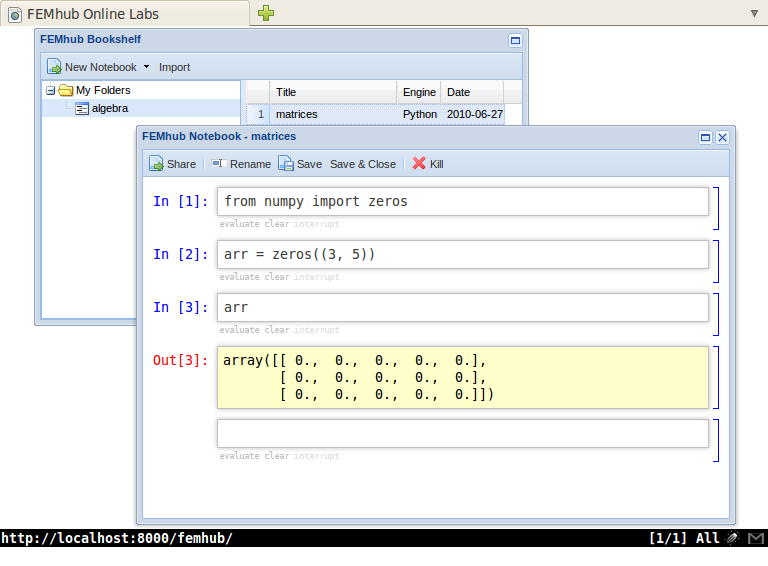
\includegraphics[scale=0.45]{images/femhub-online-lab.png}
    \end{center}
\end{frame}

%\begin{frame}
%    \frametitle{What are the missing features?}
%    \framesubtitle{}
%
%    \begin{itemize}
%        \item 3D visualisations
%            \pause
%            \begin{itemize}
%                \item can be emulated with \structure{software rendering}
%                \item \structure{preliminary support} in Firefox (canvas)
%            \end{itemize}
%        \item
%    \end{itemize}
%\end{frame}

%\begin{frame}
%    \frametitle{Future plans}
%    \framesubtitle{}
%
%    \begin{itemize}
%        \item the ultimate goal is to port programs like Agros2D to the web
%    \end{itemize}
%\end{frame}

\begin{frame}[plain]
    \begin{center}
        \textbf{Thank you for your attention!}
    \end{center}
\end{frame}

\end{document}

